\section{System Design}
\begin{figure}[h]
    \centering
    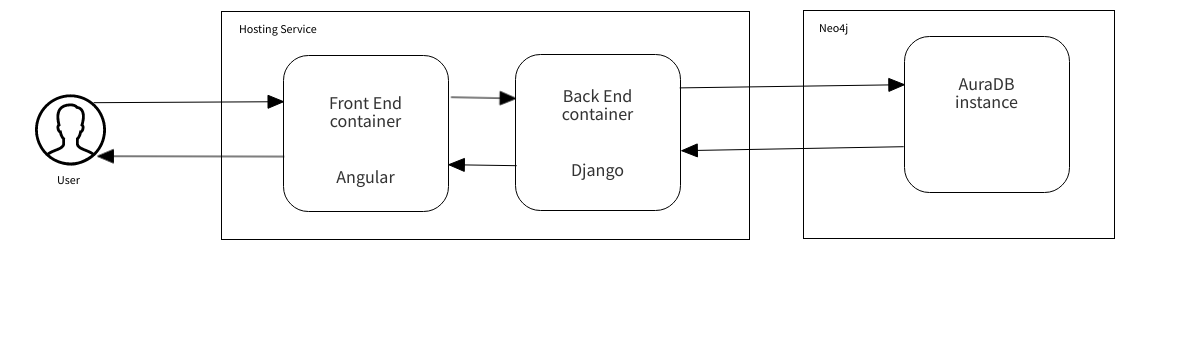
\includegraphics[scale=0.4]{system}
    \caption{System Architecture Diagram}
\end{figure}
The system architecture for this project is similar to most web based applications as the only real difference is the type of database used.
This means the user interacts with the web page created by the front end server, this then communicates with a separate back end server 
using the defined API. If needed the backend server can then communicate with the database, which in this case is hosted 
remotely by Neo4j.
The front and back end servers would likely be hosted in the cloud via the use of some containerisation system such as Docker.
\section{UI Design}
Given that the data is stored in a graph database and that is the focus of this project, it seemed obvious to display the data 
to the user as a graph. This idea was further reinforced by looking at the Neo4j tool Bloom. As shown in the screenshots below, 
Bloom is used to display the data in a dynamic and responsive graph. The main view area is called the "Scene" and just this alone allows 
the user to quickly visualise the data and see the relationships formed. In the scene the nodes can be dragged using the mouse and the graph updates 
using a physics simulation to move the other nodes. This helps ensure the other areas of the graph are still readable while still allowing the 
user to manipulate the graph.
\begin{figure}[H]
    \centering
    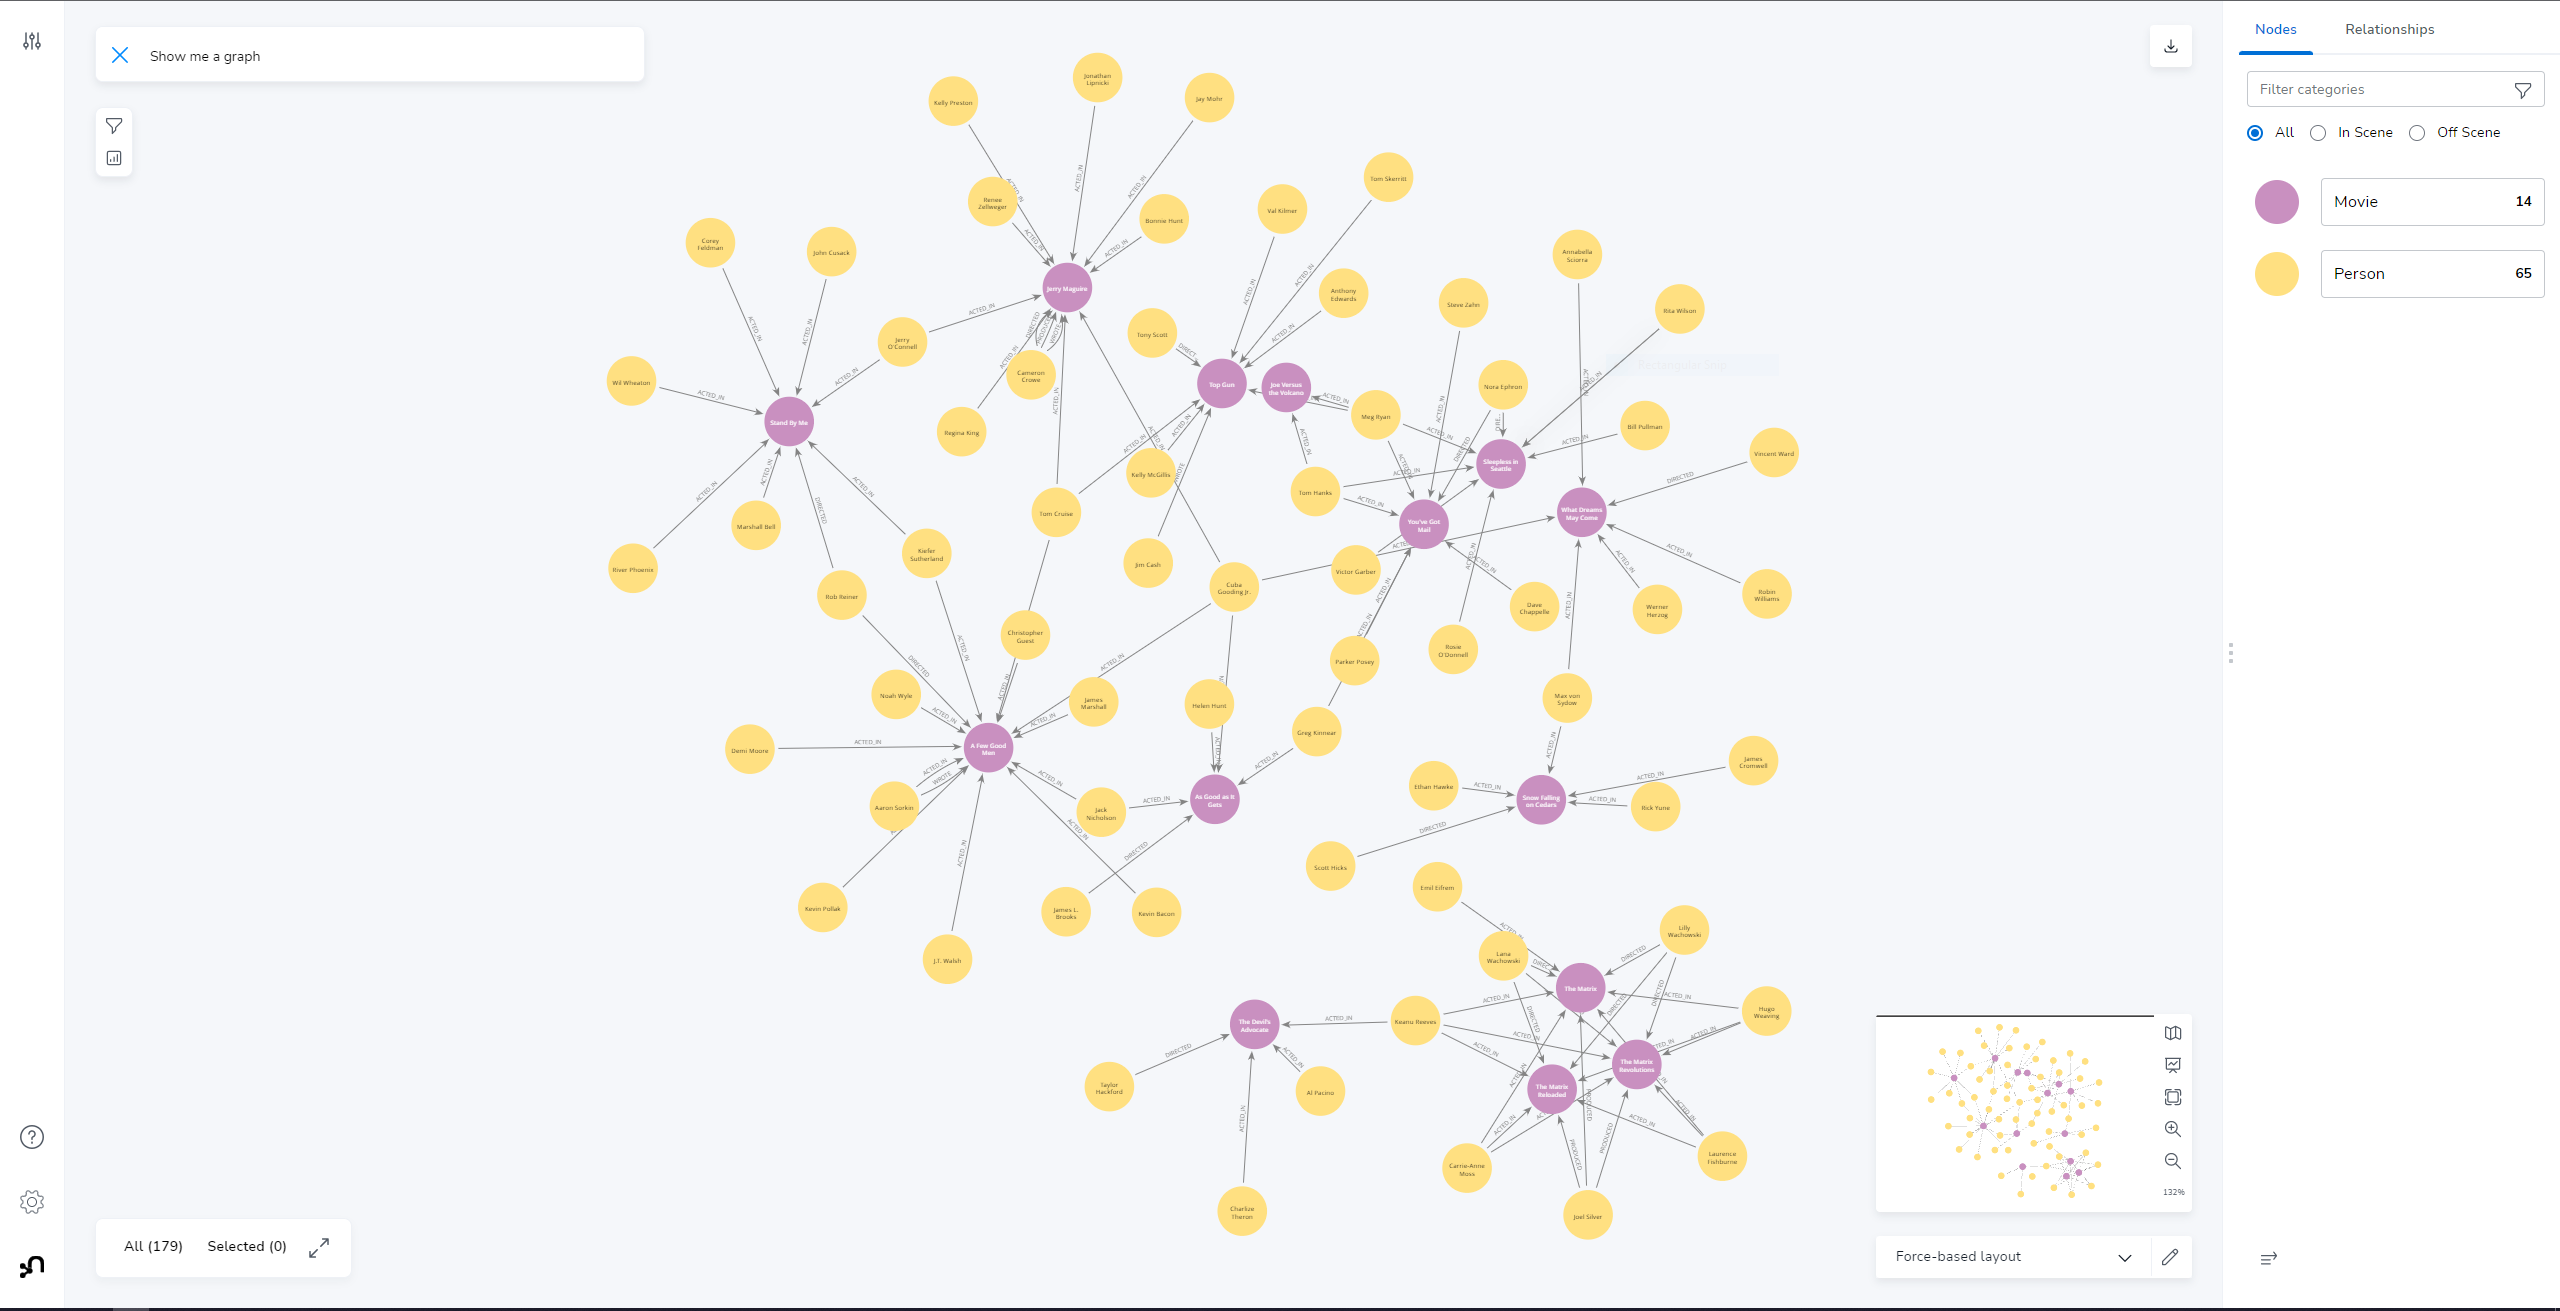
\includegraphics[width=0.8\textwidth]{bloomExample}
    \caption{Neo4j Bloom using the demo Movies database}
\end{figure}
Figure \ref{bloomImg} shows two key features of Bloom. The first is the `inspect' element which allows the user to view the full properties 
of a node or relationship by double-clicking them. This means the graph itself is not cluttered with extra information but the user can 
still easily access that data when required. The other feature is the search bar which has a few unique functions that utilise the 
graph structure of the database. It uses the types of nodes and relationships in the database to provide some quick pre-filled searches, 
For example Actor - ACTED\_IN - Movie with the demo database. This can be used to quickly filter out unwanted data from the scene without having to know 
how to write custom query statements. The second functionality follows on from this, in that the user can define their own query statements which 
become a command available in the search dropdown. This is useful if the user is familiar with Neo4j's own query language CYPHER, and they want 
to leverage that for more powerful querying.
\begin{figure}[H]%
    \centering
    \subfloat[\centering Bloom Inspect Element]{{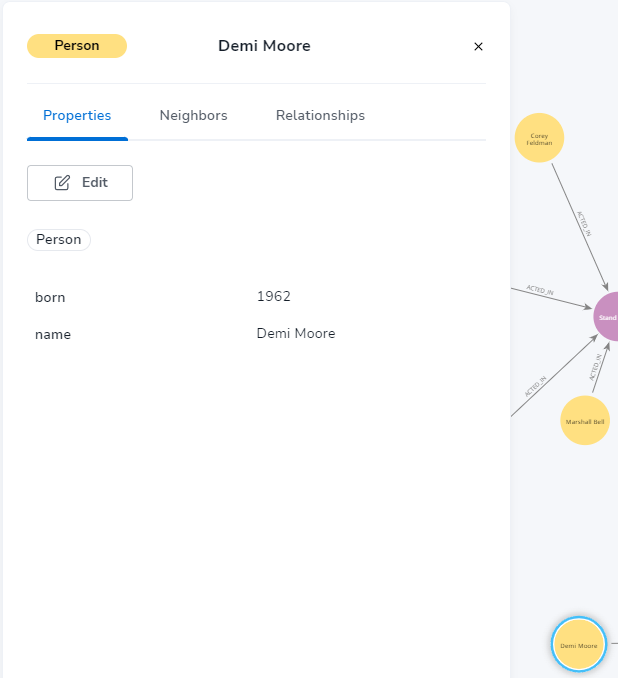
\includegraphics[width=0.4\textwidth]{images/bloomInspect.png}}}%
    \qquad
    \subfloat[\centering Bloom Search Element]{{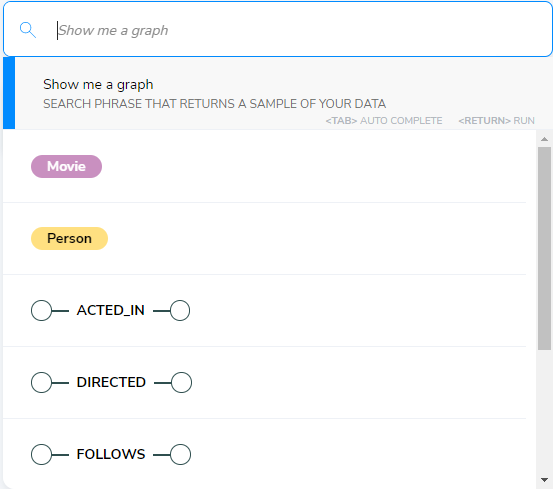
\includegraphics[width=0.4\textwidth]{images/bloomSearch.png}}}%
    \caption{Neo4j Bloom inspect and search elements}\label{bloomImg}
\end{figure}
These are all features that should be considered when implementing the user interface, however not all of them are essential for a usable application.